%!TEX program = xelatex
% Note: this template must be compiled with XeLaTeX rather than PDFLaTeX
% due to the custom fonts used. The line above should ensure this happens
% automatically, but if it doesn't, your LaTeX editor should have a simple toggle
% to switch to using XeLaTeX.

\documentclass[
  aspectratio=169, % Uncomment to use an aspect ratio of 16:9 (160 mm by 90 mm)
  %aspectratio=43, % Uncomment to use an aspect ratio of 4:3 (128mm by 96mm)
  t, % Top align all slide content by default
  onlytextwidth, % Typeset content in columns at text width
  10pt, % Default font size, use 10pt for the 16:9 aspect ratio and 8pt for the 4:3 aspect ratio
]{beamer}

\usepackage{../../ImperialTheme/beamer/beamerthemeImperial} % Use the Imperial theme
\usepackage{xcolor}
\usepackage{amsmath}
\usepackage{multirow}

\definecolor{tabpurple}{RGB}{148, 103, 189}
\definecolor{tabcyan}{RGB}{23, 190, 207}
\definecolor{tabred}{RGB}{214, 39, 40}

\def\imagefolder{../../ImperialTheme/beamer/Images}
\def\Rey{\text{Re}}
\newcommand{\qb}{\bar{q}}
\newcommand{\PhiT}{\mathcal{A}_T}

\title{Jacobian-free linear stability in Nektar++} % Presentation title to appear on the title slide and left footers


\author{Víctor Ballester and Claude} % Author name(s) to appear on the title slide

\date{\today} % Presentation date to appear on the title slide and right footers

\begin{document}

\begingroup
\setbeamercolor{background canvas}{bg=ICLLightGrey} % Slide background color
\setbeamercolor{title page title}{fg=ICLBlue} % Title text color
\setbeamercolor{title page subtitle}{fg=ICLBlue} % Subtitle text color
\setbeamercolor{author}{fg=ICLBlue} % Author(s) text color
\setbeamercolor{date}{fg=ICLBlue} % Date text color
\setbeamertemplate{title page}[logo]{\imagefolder/ICL_Logo_Blue.pdf} % Imperial logo color, use 'ICL_Logo_White.pdf' for white and 'ICL_Logo_Blue.pdf' for blue
\frame[plain, s]{\titlepage} % Output the title page with no footer ('plain') and vertically distributed text ('s')
\endgroup

%----------------------------------------------------------------------
\begin{frame}
	\frametitle{Goal and idea}
	\begin{itemize}
		\item Instead of evolving the linear operator $\mathcal{L}$, we evolve the nonlinear time stepper $\PhiT$ and approximate $\mathcal{L}$ with finite differences.
		      \[
			      \mathcal{L} v \approx \frac{\PhiT(\qb + \epsilon v) - \PhiT(\qb)}{\epsilon} \quad\text{(forward difference, 1 nonlinear run per Krylov vector)}
		      \]
		\item Validation so far:
		\begin{enumerate}
			\item Incompressible: channel flow
			\item Compressible: poiseuille flow (exact parallel flow solution), compared against Orr--Sommerfeld (local LST)
		\end{enumerate}

	\end{itemize}
\end{frame}

%----------------------------------------------------------------------
\begin{frame}
	\frametitle{Implementation (\texttt{DriverModifiedArnoldi})}
	\begin{itemize}
		\item I put \texttt{EvolutionOperator = Nonlinear}. 
		\item $\PhiT(\qb)$ is computed once at start-up and subtracted in every iteration, so a base flow that is not an exact discrete steady state does not pollute the difference. We have $\|\PhiT(\qb)-\qb\|/\|\qb\|$ $\sim 10^{-12}$ for incompressible, $10^{-10}$--$10^{-8}$ for compressible.
		\item $\epsilon$ is taken as 
		      \[
			      \epsilon\|v\| = \delta\,(1+\|\qb\|), \qquad \delta = 10^{-5},
		      \]
		      which differs from jacobain free Newton solver for the compressible solver:
		      \[
			      \epsilon\|v\| = \sqrt{\epsilon_m}\,\sqrt{(1+\|\qb\|)}, \qquad \epsilon_m = 2.22\times10^{-16}.
		      \]
      \end{itemize}
\end{frame}

%----------------------------------------------------------------------
\begin{frame}
	\frametitle{Choosing $\epsilon$ (or $\delta$ actually)}
	\begin{columns}[T]
		\begin{column}{0.49\linewidth}
			\small
			\begin{itemize}
				\item Depending on the $\delta$ chosen, the Arnoldi residual may stagnate at a floor value.
				% \item The optimal $\delta$ is problem dependent.
				\item  I do not use the Newton-solver formula because there $Jv$ only steers the step and the exact residual corrects any error at the next iteration, whereas in Arnoldi the finite difference is the operator whose eigenvalues we compute, so its error is never corrected and sets the residual floor (red square: Newton formula, stalls at $2\times10^{-6}$).
			\end{itemize}
		\end{column}
		\begin{column}{0.49\linewidth}
			\begin{figure}[ht]
				\centering
				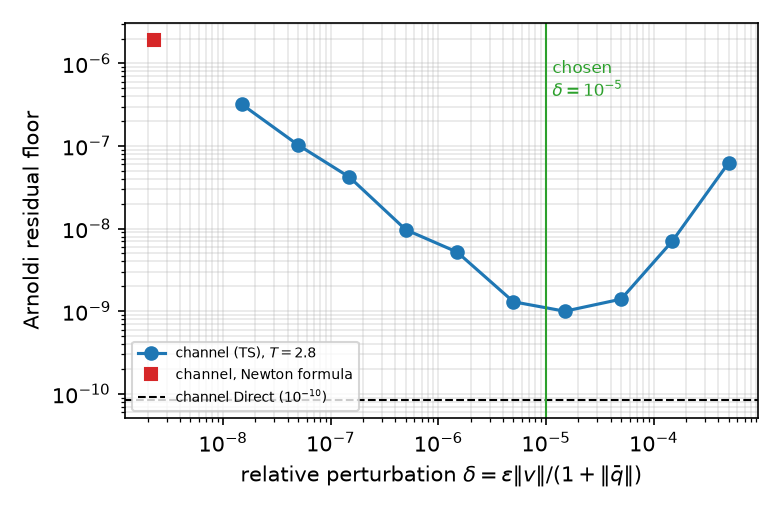
\includegraphics[width=\linewidth]{Images/epsSweep.png}
			\end{figure}
		\end{column}
	\end{columns}
\end{frame}

\begin{frame}
	\frametitle{Direct vs Nonlinear ($T=2.8$)}
	\small Reference (ref): Direct at evtol $=10^{-10}$, $\lambda = 0.769927+0.647928i$ $\Rightarrow$ growth $2.2355\times10^{-3}$, freq.\ $0.249844$.
	\vspace{-0.25cm}
	\begin{center}
		\footnotesize
		\renewcommand{\arraystretch}{1.08}
		\begin{tabular}{c@{\hspace{1.2em}}cc@{\hspace{1.2em}}cc@{\hspace{1.2em}}cc}
			\toprule
			      & \multicolumn{2}{c}{its} & \multicolumn{2}{c}{$|\lambda_a-\lambda_b|/|\lambda_{ref}|$} & \multicolumn{2}{c}{$\|\hat q_a-\hat q_b\|_\infty/\|\hat q_{ref}\|_\infty$} \\
			\cmidrule(lr){2-3}\cmidrule(lr){4-5}\cmidrule(lr){6-7}
			evtol & D & N & D vs N & N vs ref & D vs N & N vs ref \\
			\midrule
			$10^{-4}$  & 2  & 2         & $2.7\times10^{-8}$ & $2.9\times10^{-6}$ & $4.2\times10^{-5}$ & $4.9\times10^{-5}$ \\
			$10^{-5}$  & 2  & 7         & $1.5\times10^{-6}$ & $1.3\times10^{-6}$ & $1.9\times10^{-5}$ & $1.9\times10^{-5}$ \\
			$10^{-6}$  & 10 & 13        & $3.6\times10^{-7}$ & $3.8\times10^{-8}$ & $1.5\times10^{-6}$ & $2.0\times10^{-6}$ \\
			$10^{-7}$  & 19 & 24        & $2.0\times10^{-8}$ & $1.3\times10^{-8}$ & $2.3\times10^{-7}$ & $2.7\times10^{-7}$ \\
			$10^{-8}$  & 28 & 37        & $8.0\times10^{-9}$ & $5.3\times10^{-9}$ & $3.1\times10^{-8}$ & $2.8\times10^{-8}$ \\
			$10^{-9}$  & 36 & 55        & $4.7\times10^{-9}$ & $4.9\times10^{-9}$ & $1.2\times10^{-8}$ & $1.2\times10^{-8}$ \\
			$10^{-10}$ & 45 & 300$^*$   & --                 & --                 & --                 & --                 \\
			\bottomrule
		\end{tabular}
		\par\vspace{0pt}
		{$^*$not converged (300 its).}
	\end{center}
	\vspace{-0.3cm}
	\small
	\begin{itemize}
		\item Both converge to the same eigenvalue and eigenvector down to $10^{-9}$; Nonlinear needs $1.2$--$1.5\times$ iterations.
		\item $10^{-10}$ is not reachable with Nonlinear. No matter what $\delta$ I input. Central difference $O(\delta^2)$ would solve the problem, but I don't think is preferred.
	\end{itemize}
\end{frame}
%
% \begin{frame}
% 	\frametitle{Second incompressible test: Rayleigh-Bénard convection}
% 	\[
% 		\mathbf{u}_t + \mathbf{u}\cdot\nabla\mathbf{u} = -\nabla p + Pr\,\nabla^2\mathbf{u} + Ra\,Pr\,\theta\,\mathbf{e}_y,\qquad
% 		\theta_t + \mathbf{u}\cdot\nabla\theta = \nabla^2\theta,
% 	\]
% 	with BC $\mathbf{u}=0$, $\theta=1$ (bottom), $0$ (top), periodic in $x$.
% 	\begin{itemize}
% 		\item It has an exact base state $\mathbf{u}=0$, $\theta=1-y$.
% 		\item Reference: Parallel flow, local LST.
% 	\end{itemize}
% \end{frame}
%
% %----------------------------------------------------------------------
% \begin{frame}
% 	\frametitle{Nice Claude plots}
% 	\begin{columns}[T]
% 		\begin{column}{0.49\linewidth}
% 			\begin{figure}[ht]
% 				\centering
% 				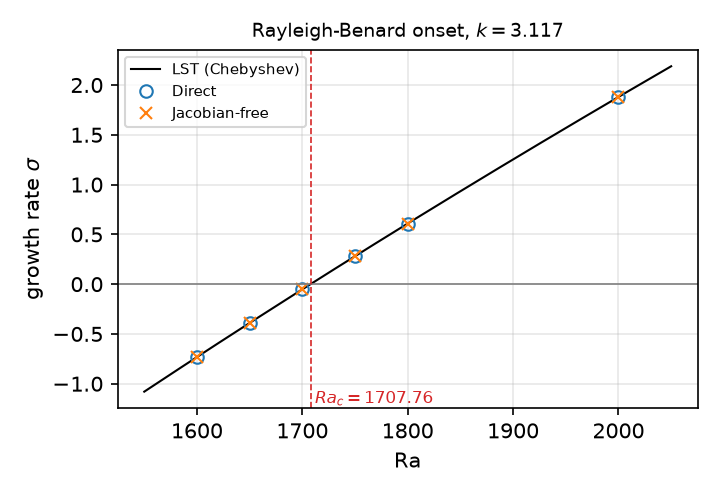
\includegraphics[width=0.85\linewidth]{Images/rb_ra.png}
% 			\end{figure}
% 			\vspace{-0.4cm}
% 			\centering\footnotesize
% 			\begin{tabular}{lc}
% 				\toprule
% 				                        & $Ra_c$ at $k=3.117$ \\
% 				\midrule
% 				Direct                  & 1707.7617           \\
% 				Jacobian-free           & 1707.7618           \\
% 				Chebyshev LST           & 1707.7619           \\
% 				Literature ($k_c=3.117$) & 1707.762           \\
% 				\bottomrule
% 			\end{tabular}
% 		\end{column}
% 		\begin{column}{0.49\linewidth}
% 			\begin{figure}[ht]
% 				\centering
% 				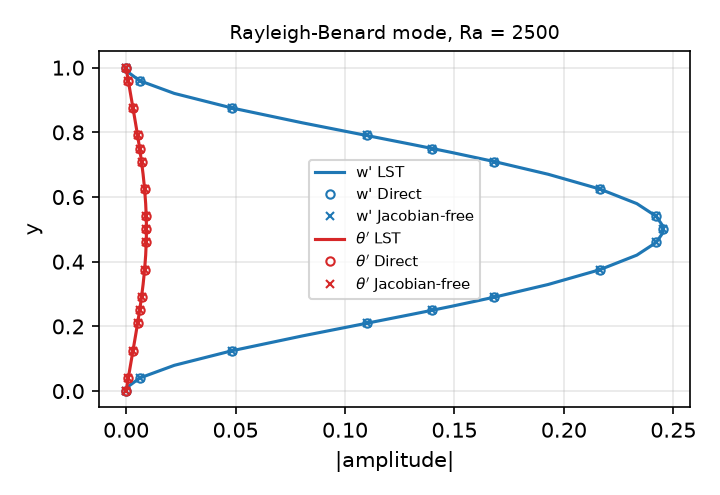
\includegraphics[width=0.85\linewidth]{Images/rb_mode.png}
% 			\end{figure}
% 			\footnotesize
% 			\begin{itemize}
% 				\item $\sigma(Ra)$ within $\sim10^{-6}$ of LST over $1600\le Ra\le2000$ ($\Delta t=1.25\times10^{-4}$).
% 				\item Eigenfunctions ($w'$, $\theta'$; $\cos kx$/$\sin kx$ amplitudes, up to a complex factor = $x$-shift): Direct vs JF $2.7\times10^{-7}$, both vs LST $\approx9\times10^{-7}$.
% 			\end{itemize}
% 		\end{column}
% 	\end{columns}
% \end{frame}
%
% %----------------------------------------------------------------------
% \begin{frame}
% 	\frametitle{Rayleigh--Bénard: time step and tolerance ($Ra=2500$)}
% 	\vspace{-0.2cm}
% 	\begin{columns}[T]
% 		\begin{column}{0.36\linewidth}
% 			\begin{figure}[ht]
% 				\centering
% 				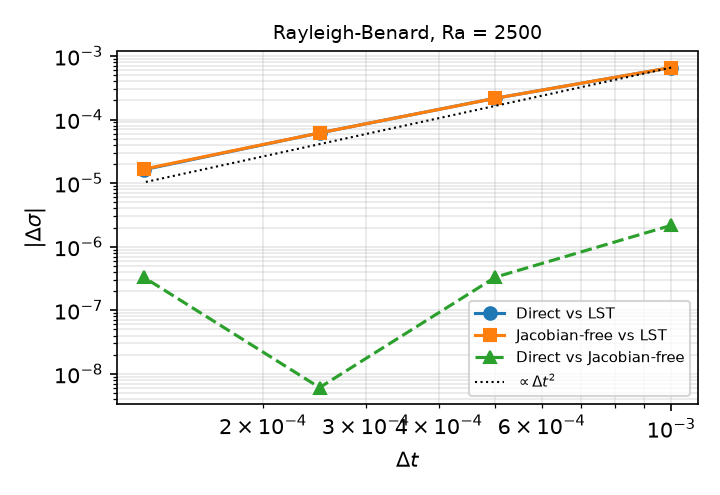
\includegraphics[height=3.3cm]{Images/rb_dt.png}
% 			\end{figure}
% 		\end{column}
% 		\begin{column}{0.62\linewidth}
% 			\begin{figure}[ht]
% 				\centering
% 				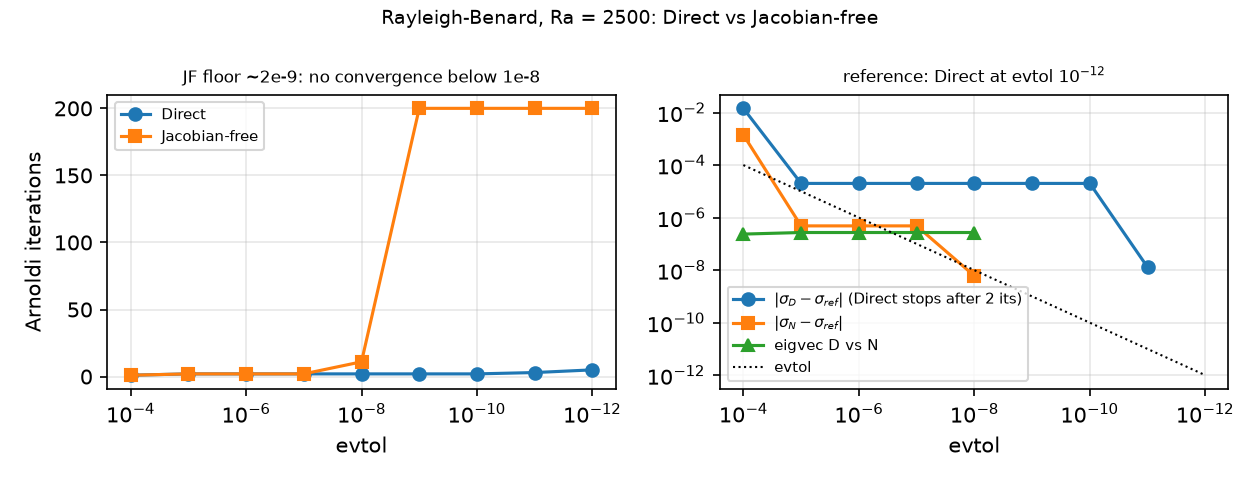
\includegraphics[height=3.3cm]{Images/rb_evtol.png}
% 			\end{figure}
% 		\end{column}
% 	\end{columns}
% 	\small
% 	\begin{itemize}
% 		\item \textbf{Gotcha}: with \texttt{nvec=1} Modified Arnoldi may stop after 2 its (Ritz estimate from a 2-vector space): Direct said residual $<10^{-9}$ but $\sigma$ was off by $2\times10^{-5}$. I first misread it as a Direct/JF mismatch. Use a tight evtol or \texttt{nvec}$\ge2$.
% 		\item JF floor $\approx2\times10^{-9}$ ($\delta=10^{-5}$): converges to evtol $10^{-8}$ (11 its), $6\times10^{-9}$ from converged Direct; not below.
% 	\end{itemize}
% \end{frame}

%----------------------------------------------------------------------
\begin{frame}
	\frametitle{Compressible case: forced plane Poiseuille}
	\small
	\begin{itemize}
		\item $\Rey=7500$, $\alpha=1$, isothermal walls ($u=v=0$, $T_w=1$) top and bottom, periodicity in $x$, constant $\mu$ and $k$, $Pr=0.72$, $\gamma=1.4$. We add a body force to the $x$-momentum ($f=2\mu$) and energy equations ($\tilde{f}=fu$).	In this conditions we have an exact equilibrium:
		      \[
			      u = 1-y^2,\quad v=0,\quad T = 1 + \tfrac{Pr(\gamma-1)M^2}{3}(1-y^4),\quad \rho = 1/T,\quad p=\text{const},
		      \]
		\item Reference: Chebyshev local LST solver for the same equations. Tends to incompressible Orr--Sommerfeld ($\lambda_{OS}=0.24989154+0.00223498i$) as for $M\to0$:
	\end{itemize}
	\begin{center}
		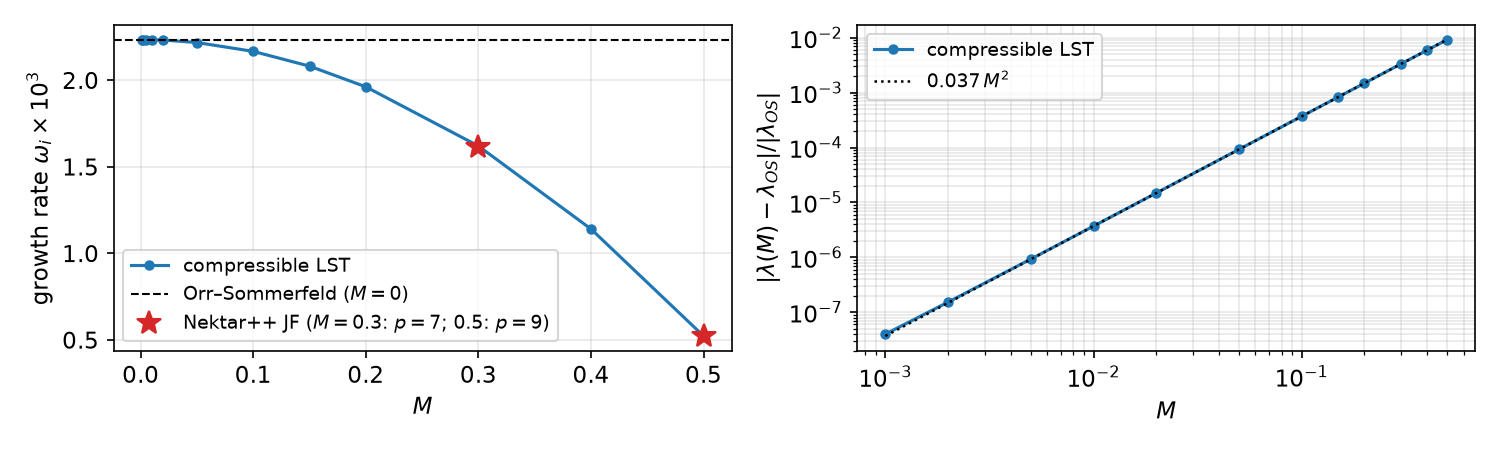
\includegraphics[height=3.4cm]{Images/machLimit.png}
	\end{center}
\end{frame}

%----------------------------------------------------------------------
% \begin{frame}
% 	\frametitle{Compressible: things that went wrong (I)}
% 	\begin{itemize}
% 		\item \textbf{LDGNS + isothermal wall is unstable.} With the default \texttt{DiffusionType=LDGNS} the base flow carries a spurious mode growing at $\sim0.1$ ($p=5$: 0.09, $p=7$: 0.14), localised in the element row next to \emph{one} wall.
% 		      \begin{itemize}
% 			      \item Seen both by Arnoldi and by a plain nonlinear run from $\qb$ + $10^{-8}$ noise (so it is not a Jacobian-free artefact).
% 			      \item Roe / HLLC / ExactToro: identical growth. Removing the energy forcing: still there. Numbering element rows from the other wall: the mode \emph{moves to the other wall}.
% 			      \item \texttt{InteriorPenalty}: gone. Probably LDG's one-sided (alternating) trace fluxes and their wall treatment. Worth reporting to the Nektar++ developers.
% 		      \end{itemize}
% 	\end{itemize}
% \end{frame}

%----------------------------------------------------------------------

%----------------------------------------------------------------------
\begin{frame}
	\frametitle{Compressible results: Jacobian-free Arnoldi vs LST}
	\vspace{0.2cm}
	\begin{columns}[T]
		\begin{column}{0.5\linewidth}
			\centering
			\renewcommand{\arraystretch}{1.15}
			\begin{tabular}{ccc@{\hspace{1em}}c@{\hspace{1.2em}}c}
				\toprule
				$M$ & $p$ & its & $\dfrac{|\lambda_N-\lambda_{LST}|}{|\lambda_{LST}|}$ & $\dfrac{\|\hat q_N-\hat q_{LST}\|_\infty}{\|\hat q_{LST}\|_\infty}$ \\
				\midrule
				\multirow{5}{*}{0.5}
				    & 5 & 32 & $2.7\times10^{-3}$ & $1.4\times10^{-2}$ \\
				    & 6 & 31 & $6.2\times10^{-4}$ & $4.8\times10^{-3}$ \\
				    & 7 & 30 & $1.0\times10^{-4}$ & $1.1\times10^{-3}$ \\
				    & 8 & 30 & $3.5\times10^{-5}$ & $2.7\times10^{-4}$ \\
				    & 9 & 20 & $6.8\times10^{-6}$ & $8.7\times10^{-5}$ \\
				\midrule
				0.3 & 7 & 26 & $1.0\times10^{-4}$ & $1.0\times10^{-3}$ \\
				\bottomrule
			\end{tabular}
		\end{column}
		\begin{column}{0.48\linewidth}
			\centering
			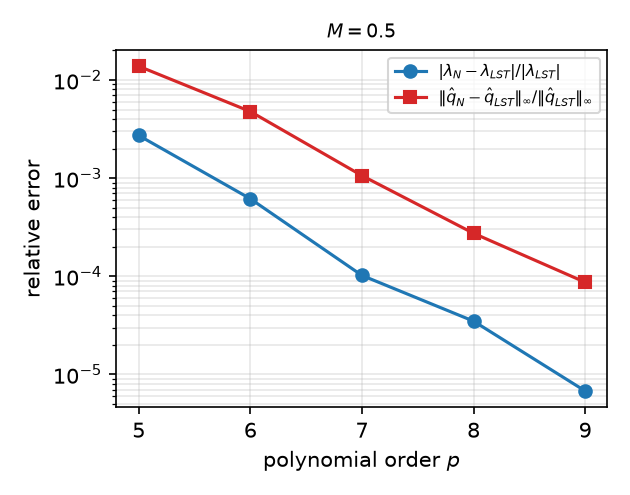
\includegraphics[width=0.92\linewidth]{Images/compErr.png}
		\end{column}
	\end{columns}
	\vspace{0.05cm}
	\footnotesize
	$\lambda=\omega_r+i\,\omega_i$: complex eigenvalue (frequency + growth). $\hat q=(\rho',u',v',T')$. evtol $=10^{-6}$, $T=28$.
\end{frame}

%----------------------------------------------------------------------
\begin{frame}
	\frametitle{Compressible TS eigenfunctions}
	\begin{figure}[ht]
		\centering
		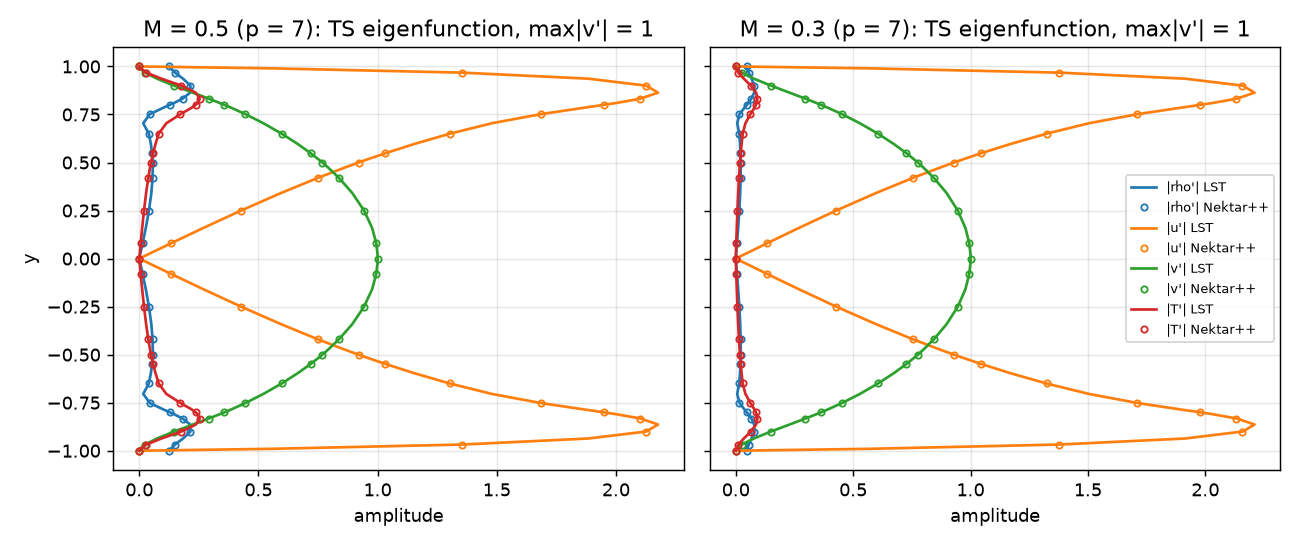
\includegraphics[width=\textwidth]{Images/modes.png}
	\end{figure}
\end{frame}

\end{document}
